\documentclass[french, handout]{beamer}
\usepackage[utf8]{inputenc}
\usepackage[T1]{fontenc}
\usepackage[french]{babel}
\usepackage[squaren,Gray,cdot]{SIunits}
\usepackage{tcolorbox}
\usepackage[absolute,overlay]{textpos}
\usepackage{svg}
\usepackage{hyperref}
\usetheme{Warsaw}

\renewcommand{\per}{\reciprocal}
\DeclareMathOperator{\cotan}{cotan}

\setbeamertemplate{itemize item}[ball]
\setbeamertemplate{headline}{}
\setbeamertemplate{footline}{
    \leavevmode%
        \hbox{\hspace*{-0.1cm}
        \begin{beamercolorbox}[wd=.2\paperwidth,ht=2.25ex,dp=1ex,center]{author in head/foot}%
        	\usebeamerfont{author in head/foot}\insertshortauthor%~~(\insertshortinstitute)
        \end{beamercolorbox}
        \begin{beamercolorbox}[wd=.6\paperwidth,ht=2.25ex,dp=1ex,center]{section in head/foot}%
        	\usebeamerfont{section in head/foot}\insertshorttitle
        \end{beamercolorbox}
        \begin{beamercolorbox}[wd=.2\paperwidth,ht=2.25ex,dp=1ex,center]{section in head/foot}%
        	\usebeamerfont{section in head/foot}
        	\insertframenumber{} / \inserttotalframenumber\hspace*{2ex}
        \end{beamercolorbox}
}}
\AtBeginSection[]
{
\begin{frame}{Sommaire}
    \tableofcontents[currentsection, hideothersubsections]
\end{frame}
}


\title[Commande de direction automatisée d'un véhicule]{Automatisation de la commande de direction d'un véhicule}
\subtitle{Réalisation d'un prototype adaptant sa position en fonction de son environnement}
\author{Henri Lasserre}
\date{TIPE : 2017-2018}
\institute{}


\begin{document}
    
    \begin{frame}
        \titlepage
    \end{frame}
    
    \begin{frame}{Sommaire}
        \tableofcontents[hideothersubsections]
    \end{frame}
    
    \section{Introduction}
%%%%%%%%%%%%%%%%
% Introduction %
%%%%%%%%%%%%%%%%
        \begin{frame}{Introduction}
            \begin{block}{Problématique}
            \begin{itemize}
                \item \quad Comment réaliser un véhicule semi-autonome, capable de s'orienter et de suivre un chemin prédéfini, adaptant sa vitesse en fonction des conditions environnementales dans lesquelles il évolue ?
                \item \quad Comment optimiser les commandes des systèmes afin de garantir la sécurité des passagers et minimiser le temps de trajet ? 
            \end{itemize}
            \end{block}
            
        \end{frame}
        
%%%%%%%%%%%%%%%%
% Présentation %
%%%%%%%%%%%%%%%%
        \begin{frame}{Présentation du système}
        \begin{figure}
            \centering
            \includesvg[width=10.5cm]{pres_systeme.svg}
        \end{figure}
        \end{frame}
        
        \begin{frame}{Présentation du système}
            \begin{figure}
                \hspace*{-2em}
                \includegraphics[scale=0.35]{magicDrawBDD.png}
                \caption{Diagramme de définition de blocs}
            \end{figure}
        \end{frame}
        
        \begin{frame}{Présentation du système}
        \framesubtitle{\quad Schéma d'architecture fonctionnelle}
        \begin{figure}[htbp]
          \centering
          \includesvg[scale=.33]{ibd.svg}
          \caption{Diagramme de la chaîne fonctionnelle du système}
        \end{figure}
        \end{frame}
        
        \begin{frame}{Présentation de l'objectif}
        \framesubtitle{Environnement à maîtriser}
        \begin{figure}[htbp]
          \centering
          \includesvg[scale=.4]{parcours.svg}
          \caption{Parcours à réaliser par la voiture}
        \end{figure}
        \end{frame}
    
%%%%%%%%%%%%%%%%%%%%%%%%%%
% Caractéristiques moteur %
%%%%%%%%%%%%%%%%%%%%%%%%%%
    \section{Caractéristiques des capteurs et actionneur}
        
        \subsection{Motoréducteur}
        \begin{frame}
        \frametitle{Sommaire}
        \tableofcontents[sections=2, currentsubsection]
        \end{frame} 
        
        \begin{frame}{\hyperlink{details_moteur}{Motoréducteur}}
        \label{pres_moteur}
            \vspace{-0.2cm}
            \begin{block}{Moteur et équations}
                \begin{columns}[c]
                    \begin{column}{3 cm}
                        \includegraphics[width=2.9cm]{motoreducteur_ferme.jpg}
                    \end{column}
                    \hspace{-0.3cm}
                    \begin{column}{7 cm}
                        \begin{tcolorbox}[colback=red!5!white, colframe=red!75!black, title=Équations du MCC]
                            {\footnotesize \[ \left\{
                                    \begin{aligned}
                                    &U=RI+L\frac{dI}{dt}+E\\
                                    &C=K_{i}I\\
                                    &E=K_{e}\omega\\
                                    &J_{eq}\frac{d\omega}{dt}=C_{m}-C_{r}-f\omega
                                    \end{aligned}
                                    \right. \]}
                        \end{tcolorbox}
                    \end{column}
                \end{columns}
            \end{block}
            \vspace{-0.1cm}
            \begin{block}{Caractéristiques mesurées}
                \centering
                \begin{columns}[c]
                \begin{column}{3 cm}
                    \vspace{-.5cm}
                    \begin{figure}[htbp]
                      \centering
                      \includesvg[height=2.1cm]{reducteur.svg}
                    \end{figure}
                \end{column}
                \begin{column}{7.5 cm}
                    \begin{tabular}{ | c | c | c | c | }
                        \hline
                         R ($\Omega$)&L(mH)&Ke (\volt\usk\per\radian)&r\\ \hline
                         8,47& 19,0 & 4,4\cdot10\up{-3} & 0,005 \\
                         \hline
                    \end{tabular}
                \end{column}
            \end{columns}
            \end{block}
        \end{frame}
    
    \subsection{Étalonnage des capteurs}
    
    \begin{frame}
    \frametitle{Sommaire}
    \tableofcontents[sections=2, currentsubsection]
    \end{frame} 
    
    \begin{frame}{Étalonnage des capteurs}
        \label{pres_capteurs}
        \begin{block}{\hyperlink{details_ultrason}{Capteur à ultrason}}
            \begin{columns}
                \begin{column}{5cm}
                \includegraphics[width=5cm]{Etalonage_capteur_distance.png}
                \end{column}
                \begin{column}{5cm}
                    \centering
                    On a donc : \hspace{1.5\baselineskip}\fbox{$d=\frac{\Delta t}{58}$ cm.}
                \end{column}
            \end{columns}
        \end{block}
        \begin{block}{\hyperlink{details_pot}{Capteur potentiométrique}}
            \begin{columns}
            \begin{column}{5cm}
                \includegraphics[width=5cm]{CAN-angle_etalonnage_pot.png}
                \end{column}
                \begin{column}{5cm}
                    On a donc : \fbox{$n=12.49\times \theta + 510$}
                \end{column}
            \end{columns}
        \end{block}
    \end{frame}
%%%%%%%%%%%%%%%%%%%%%%%
% Modélisations %
%%%%%%%%%%%%%%%%%%%%%%%    
    \section{Modélisations du système}
    \subsection{Modélisation SolidWorks}
    
    \begin{frame}
    \frametitle{Sommaire}
    \tableofcontents[sections=3, currentsubsection]
    \end{frame} 
    
    \begin{frame}{Modélisation SolidWorks}
        \begin{figure}
            \centering
            \includegraphics[width=11cm]{vue_sd_perspective.png}
            \caption{Modélisation sous SolidWorks du train avant du véhicule}
        \end{figure}
    \end{frame}
    \begin{frame}{Modélisation SolidWorks}
        \begin{figure}
            \centering
            \includegraphics[height=4cm]{inertie.png}
            \caption{Inertie équivalente ramenée sur l'arbre de sortie du réducteur en fonction du temps}
        \end{figure}
        \begin{block}{Valeur de l'inertie}
        \centering
            Si $J_m=\langle J(t)\rangle=6,5\cdot10^{-6}\kilogram\usk\meter\squared$, alors :~\fbox{$J_{eq}=J_m\times r^2=1,6\cdot10^{-8}\kilogram\usk\meter\squared$}
        \end{block}
    \end{frame}
    
    \subsection{Modélisation Matlab}
    
    \begin{frame}
    \frametitle{Sommaire}
    \tableofcontents[sections=3, currentsubsection]
    \end{frame} 
    
    \begin{frame}{Modélisation Matlab}
        \begin{figure}
            \centering
            \includegraphics[width=11cm]{schema_bloc.png}
            \caption{Schéma-bloc du système modélisé}
        \end{figure}
    \end{frame}

%%%%%%%%%%%%%%%%%%%%%
% Création du systeme %
%%%%%%%%%%%%%%%%%%%%%    
    \section{Mesures expérimentales sur le système}

% Mise en place de l'asservissement %            
        \subsection{Mise en place d'un asservissement}
        
        \begin{frame}
        \frametitle{Sommaire}
        \tableofcontents[sections=4, currentsubsection]
        \end{frame}
        
            \begin{frame}{Asservissement de position}
            \begin{block}{Protocole suivi}
            \begin{itemize}
                \item Position initiale 300, consigne 700;
                \item A chaque instant : \begin{itemize}
                    \item \textbf{Acquisition} potentiomètre
                    \item Calcul de l'\textbf{écart} (proportionnel), de la \textbf{somme des écarts} (intégral), de la \textbf{différence des écarts} (dérivé);
                    \item Calcul du \textbf{rapport cyclique} (avec les gains du PID);
                    \item \textbf{Normalisation} du rapport cyclique (butée, plage possible, sens de déplacement);
                \end{itemize}
                \item \textbf{Modification des gains} et comparaison des différents essais.
                \item \textbf{Conclusion} : meilleures performances;
            \end{itemize}
            \textbf{Remarque} : FTBO de classe 1 (asservissement de position)$\Rightarrow$ erreur statique nulle $\Rightarrow$ correcteur intégral inadapté (confirmé expérimentalement).
            \end{block}
            \end{frame}
            
            \begin{frame}{Correcteur proportionnel}
                \begin{figure}
                    \centering
                \hspace*{-4.2em}
                    \includegraphics[width=14cm]{deter_kp.png}
                \end{figure}
            \end{frame}
            
            \begin{frame}{Correcteur dérivé}
                \begin{figure}
                    \centering
                    \hspace*{-4.2em}
                    \includegraphics[width=14cm]{deter_kd.png}
                \end{figure}
            \end{frame}
            
        \subsection{Utilisation pour un positionnement}
        \begin{frame}
        \frametitle{Sommaire}
        \tableofcontents[sections=4, currentsubsection]
        \end{frame}
        \begin{frame}{Positionnement du véhicule sur la chaussée}
            \begin{figure}
                \centering
                \includegraphics[scale=0.8]{loi_commande.png}
            \end{figure}
        \end{frame}
        
        \begin{frame}{Positionnement du véhicule : objectif et protocole}
            \begin{block}{Objectif}
                Déplacer le véhicule au milieu de la route.
            \end{block}
            \begin{block}{Protocole}
            \begin{figure}
                \centering
                \includesvg[height=5cm]{3mesures_init.svg}
            \end{figure}
            \end{block}
        \end{frame}
        
        \begin{frame}{Positionnement du véhicule sur la chaussée}
            \begin{figure}
                \centering
                \hspace*{-4.2em}
                \includegraphics[width=14cm]{couloir_voiture_temporel.png}
            \end{figure}
        \end{frame}
        
        \begin{frame}{Positionnement du véhicule sur la chaussée}
            \begin{figure}
                \centering
                \hspace*{-4.2em}
                \includegraphics[width=14cm]{parcours_voiture_temporel.png}
            \end{figure}
        \end{frame}
        
        \subsection{Utilisation pour un virage}
        \begin{frame}
        \frametitle{Sommaire}
        \tableofcontents[sections=4, currentsubsection]
        \end{frame}
        \begin{frame}{Utilisation pour un virage}
            \begin{block}{Hypothèses}
            \begin{itemize}
                \item Direction du virage connue à l'avance;
                \item Voiture initialement au milieu de la route;
                \item Route identique avant et après le virage (même largeur).
            \end{itemize}
            \end{block}
            \begin{block}{Théorie}
            \begin{itemize}
                \item Relation entre le rayon de courbure $R$, l'angle de braquage des roues $\theta$, et l'empattement $\delta$ de la voiture : 
                \[\fbox{$\tan(\theta) = \frac{\delta}{R}$}\]
                \item Avec $\theta$ défini par : \[\fbox{$\theta=\arctan\left(\frac{2}{\cotan(\theta_e)+\cotan(\theta_i))}\right)$}\]
            \end{itemize}
            \end{block}
        \end{frame}
        
    \section{Comparaison des résultats et conclusion}
    \begin{frame}{Comparaison des résultats}
        \begin{figure}
            \centering
            \includegraphics[width=11cm]{exp_theo_kp2.png}
        \end{figure}
    \end{frame}
    \begin{frame}{Conclusion}
    Ce TIPE m'a demandé d'adopter la démarche d'un ingénieur. En effet j'ai :
    \begin{itemize}
        \item Transposé un objectif qualitatif en objectif quantitatif;
        \item Caractérisé les outils à ma disposition (caractéristiques techniques et physiques);
        \item Modélisé le système désiré;
        \item Réalisé réellement le système;
        \item Comparé les deux résultats obtenus.
    \end{itemize}
        
    \end{frame}
    
    \section{Annexe}
        \begin{frame}{\hyperlink{pres_moteur}{Moteur à courant continu}}
        \label{details_moteur}
            \vspace{-0.2cm}
            \begin{block}{Moteur et équations}
                \begin{columns}[c]
                    \begin{column}{3 cm}
                        \includegraphics[width=2.9cm]{motoreducteur.jpg}
                    \end{column}
                    \hspace{-0.3cm}
                    \begin{column}{7 cm}
                        \begin{tcolorbox}[colback=red!5!white, colframe=red!75!black, title=Équations du MCC]
                            {\footnotesize \[ \left\{
                                    \begin{aligned}
                                    &U=RI+L\frac{dI}{dt}+E\\
                                    &C=K_{i}I\\
                                    &E=K_{e}\omega\\
                                    &J_{eq}\frac{d\omega}{dt}=C_{m}-C_{r}-f\omega
                                    \end{aligned}
                                    \right. \]}
                        \end{tcolorbox}
                    \end{column}
                \end{columns}
            \end{block}
            \vspace{-0.1cm}
            \begin{block}{Réducteur}
                \begin{columns}[c]
                    \begin{column}{3.5 cm}
                        \vspace{-.75cm}
                        \begin{figure}[htbp]
                          \centering
                          \includesvg[height=2.3cm]{reducteur.svg}
                        \end{figure}
                    \end{column}
                    \hspace{-0.7cm}
                    \begin{column}{6.5 cm}
                        \begin{tcolorbox}[colback=red!5!white, colframe=red!75!black, title=Equation : Rapport de réduction]
                            {\footnotesize \[r= \frac{15\times10\times10\times17}{70\times50\times35\times41} = 0.005\]}
                        \end{tcolorbox}
                    \end{column}
                \end{columns}
            \end{block}
        \end{frame}
        
% Détermination de R %
            \begin{frame}{\hyperlink{pres_moteur}{Détermination de R}}
                \begin{block}{Essai à rotor bloqué}
                    \begin{columns}[c]
                    
                        \begin{column}{5 cm}
                            \includegraphics[width=6 cm, height = 3.5 cm]{tension-courant_deter_R.png}
                        \end{column}
                    
                        \begin{column}{4.5 cm}
                            \begin{tcolorbox}[colback=red!5!white,colframe=red!75!black,title=Equation]
                                \begin{center}
                                    \fcolorbox{red}{red!5!white}{$U=R\times I$} 
                                \end{center}
                            \end{tcolorbox}
                            \begin{tcolorbox}[colback=green!5!white,colframe=green!75!black,title=Résultat]
                                \[R=8,47~ \Omega\]
                            \end{tcolorbox}
                        \end{column}
                    \end{columns}
                \end{block}
            \end{frame}

% Détermination de L %
            \begin{frame}{\hyperlink{pres_moteur}{Détermination de L}}
                \begin{block}{Intensité moteur au démarrage}
                    \begin{columns}[c]
                    
                        \begin{column}{5 cm}
                            \includegraphics[width=6 cm, height = 3.5 cm]{courant-temps_deter_L.png}
                            \vspace{0.1cm}
                            \begin{tcolorbox}[text width = 4.9cm, colback=green!5!white, colframe=green!75!black, title=Résultat]
                                \[L=19,0~ \milli\henry\]
                            \end{tcolorbox}
                        \end{column}
                    
                        \begin{column}{4.5 cm}
                            \begin{tcolorbox}[text height = 4.2 cm, colback=red!5!white, colframe=red!75!black, title=Equation]
                               \begin{center}
                                   \fcolorbox{red}{red!5!white}{\small $I(t)=I_{0}(1-\exp(\frac{-t}{\tau}))$} 
                                    ~\\ $\begin{aligned} &Avec : \\&\left\{
                                    \begin{aligned}
                                    &I_{0}=1.035 \, \ampere\\
                                    &\tau=\frac{L}{R}=0.16 \, \milli\second
                                    \end{aligned}
                                    \right.\end{aligned} $ 
                               \end{center} 
                            \end{tcolorbox}
                        \end{column}
                    \end{columns}
                \end{block}   
            \end{frame}

% Détermination de Ke %
            \begin{frame}{\hyperlink{pres_moteur}{Détermination de $K_e$}}
                \begin{block}{Essai en régime permanent}
                    \begin{columns}[c]
                        \begin{column}{4.1cm}
                             \begin{tcolorbox}[colback=red!5!white, colframe=red!75!black, title=Equation]
                                \small{$ \left\{
                                    \begin{aligned}
                                    &K_{e}=\frac{E}{\omega}\\
                                    &E=U-RI
                                    \end{aligned}
                                    \right.$}
                                \\Donc \large{\fcolorbox{red}{red!5!white}{$K_{e}=\frac{U-RI}{\omega}$}}
                            \end{tcolorbox}
                        \end{column}
                        \hspace{-0.8cm}
                        \begin{column}{6.5cm}
                            \begin{tabular}{ | c | c | c | c | }
                                \hline
                                 U (\volt)& I (\ampere)& R ($\Omega$)& $\omega$ (\radian\usk\per\second)\\ \hline
                                 1  & 0,04 & 8,47 & 151 \\
                                 \hline
                            \end{tabular}
                            \vspace{0.4cm}
                            \begin{tcolorbox}[text width = 4.6cm, colback=green!5!white, colframe=green!75!black, title=Résultat]
                                $K_{e}=4,4\cdot 10^{-3}~ \volt\usk\per\radian$
                            \end{tcolorbox}
                        \end{column}
                    \end{columns}
                \end{block}
            \end{frame}
            

% Mesure de distance %
            \begin{frame}{\hyperlink{pres_capteurs}{Capteur ultrason}}
            \label{details_ultrason}
            \framesubtitle{\quad Implémentation sur la voiture}
                \vspace{-0.1cm}
                \begin{center}
                    \hspace*{-0.5em}
                    \fbox{\includegraphics[scale=0.06]{voiture_lateral.jpg}}
                \end{center}
            \end{frame}
            \begin{frame}{\hyperlink{pres_capteurs}{Mesure de distance}}
            \framesubtitle{\quad Présentation du capteur}
                    \begin{columns}[c]
                        \hspace{-1.2cm}
                        \begin{column}{4cm}
                            \includegraphics[width=4.7cm]{capteur_distance.png}\\
                            \includegraphics[width=4.75cm]{distance.jpg}
                        \end{column}
                        \begin{column}{5cm}
                            \begin{tcolorbox}[text width = 5cm, colback=gray!5!white,colframe=gray!75!black, title=Objectif et protocole]
                                    \quad Déterminer une \textbf{relation} reliant \textbf{l’information renvoyée par le capteur} et \textbf{la distance séparant l’objet du capteur}.
                                    \tcblower
                                    \quad Relever les données \textbf{renvoyées par la carte} et \textbf{la distance séparant l’objet du capteur}.\\
                                    \quad Déterminer \textbf{la loi reliant les deux données}. 
                            \end{tcolorbox}
                        \end{column}
                    \end{columns}
            \end{frame}
            \begin{frame}{\hyperlink{pres_capteurs}{Mesure de distance}}
            \framesubtitle{\quad Résultats et conclusion}
            \begin{center}
                \includegraphics[height=3.8cm]{Etalonage_capteur_distance.png}
                \begin{tcolorbox}[colback=green!5!white, colframe=green!75!black, title=Résultat]
                    \quad \underline{Coefficient directeur :} \quad \fcolorbox{red}{green!5!white}{$a=\frac{1}{58}~\centi\meter\usk\micro\per\second$}
                \end{tcolorbox}
            \end{center}
            \end{frame}

% Mesure de position %
            \begin{frame}{\hyperlink{pres_capteurs}{Capteur potentiométrique}}
            \label{details_pot}
                \begin{columns}[c]
                    \hspace{0.1cm}
                    \begin{column}{6cm}
                        \includegraphics[width=7cm]{CAN-angle_etalonnage_pot.png}\\
                        \includesvg[width=7cm]{angles_differents.svg}
                    \end{column}
                    \hspace{1.1cm}
                    \begin{column}{6cm}
                        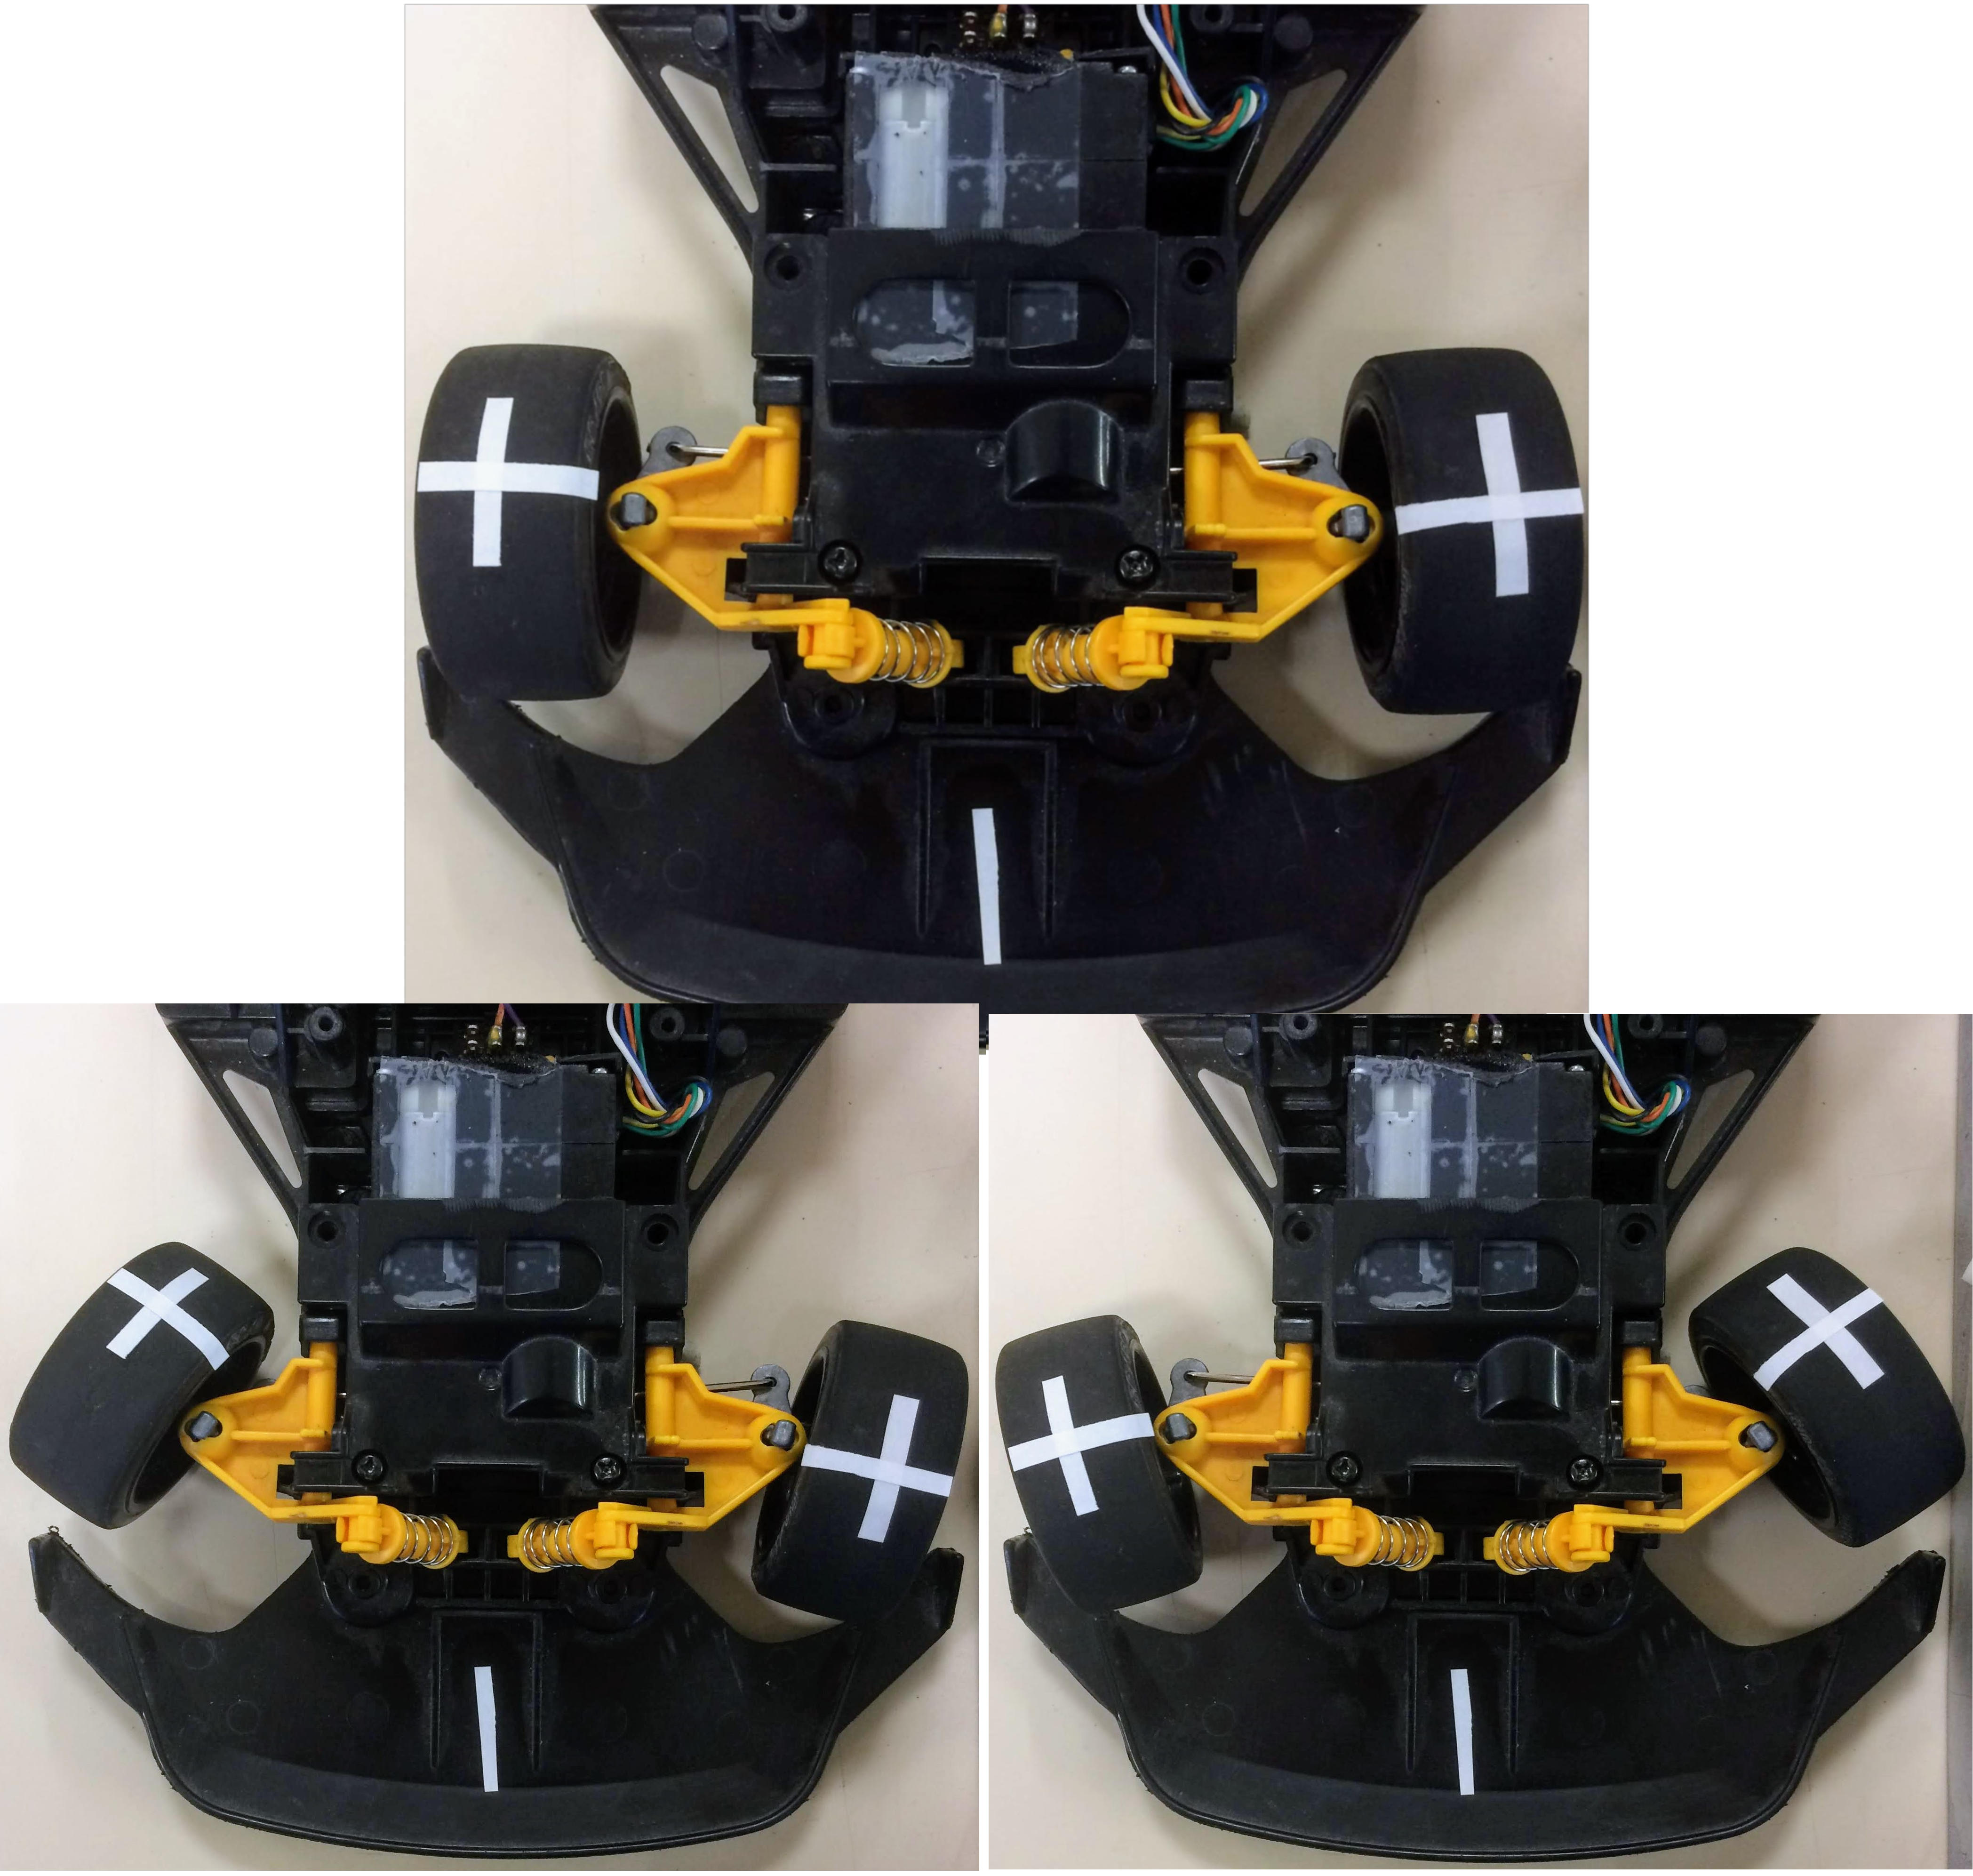
\includegraphics[width=5cm]{montage_angle_roues.png}
                    \end{column}
                \end{columns}
            \end{frame}

% Commande du moteur %
            \begin{frame}{Hacheur 4 quadrants}
            \framesubtitle{\quad Présentation du L298N}
                    \begin{center}
                    \begin{columns}[c]
                        \begin{column}{5cm}
                            \fbox{\includegraphics[width=4cm]{l298n.png}}
                        \end{column}
                        \begin{column}{5cm}
                            \fbox{\includegraphics[width=4cm]{l298n2.jpg}}
                        \end{column}
                    \end{columns}
                    \vspace{0.5cm}
                    \fbox{\includegraphics[width = 7.5 cm]{moteur_sens.png}}
                    \end{center}
            \end{frame}
\end{document}